\newpage
\rhead{\textbf{\textcolor{blue}{Т}\textcolor{gray}{ерминология: информация и данные}}}
\makebox[0pt][l]{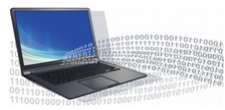
\includegraphics[scale=0.5]{img/pic.png} }
\vspace*{2mm}
\newline
\begin{flushleft}
 Международный стандарт ISO/IEC 2382:2015\\
«Information technology – Vocabulary» (вольный пересказ):\\
\qquad \textcolor{Green}
{Информация} – знания относительно фактов, событий, \\ \qquad вещей, идей и  понятий.
\\
		\qquad \textcolor{Green}{Данные} – форма представления информации в виде, \\ \qquad пригодном для передачи или обработки. \\
\end{flushleft}
	\vspace*{3mm}
	\textbullet \ Что есть предмет информатики: информация или данные? \\
	\textbullet \ Как измерить информацию? Как измерить данные? 	Пример: «Байкал — самое глубокое озеро Земли».
	